\section{The indexing architecture}
\subsection{Statistical Properties of Text}
\begin{itemize}
    \item Zipf's law: frequency of word is inversely proportional to its rank (deviates for high frequency and low frequency words)
    \item Heaps' law: number of unique words is sublinear in number of words in collection
\end{itemize}
\subsection{Text analysis pipeline}
\begin{enumerate}
    \item remove whitespace and punctuation
    \item convert terms to lower-case
    \item remove stop-words (words that occur in every document -> are not characteristic for document)
    \item convert terms to stems (e.g. drop suffixes etc.)
    \item deal with phrases
\end{enumerate}
\begin{itemize}
    \item how to determine that word is stop word?: either through frequency threshold or by using dictionary (or using a combination of both)
    \item different approaches to stemming:
    \begin{itemize}
        \item porter stemmer is a list of manually created rules
        \item dictionary-based stemming: has new-words problems
        \item hybrid approach (e.g. krovetz stemmer). uses dictionary-based approach first. if word is not found -> apply algorithmic stemmer -> check dictionary again -> if not found again apply rule and check dictionary again ...
    \end{itemize}
\end{itemize}
\subsection{Web graph}
\begin{figure}[ht]
    \centering
    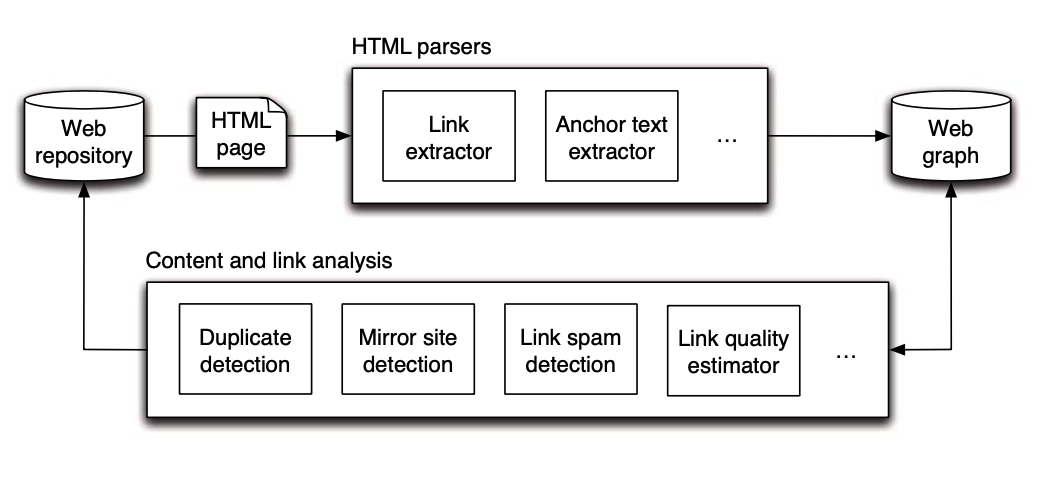
\includegraphics[width=0.7\textwidth]{figures/web_graph.png}
    \caption{Web graph}
\end{figure}
\begin{itemize}
    \item see collection as graph where documents are nodes and links are edges
\end{itemize}
\subsection{Forward index}
\begin{figure}[ht]
    \centering
    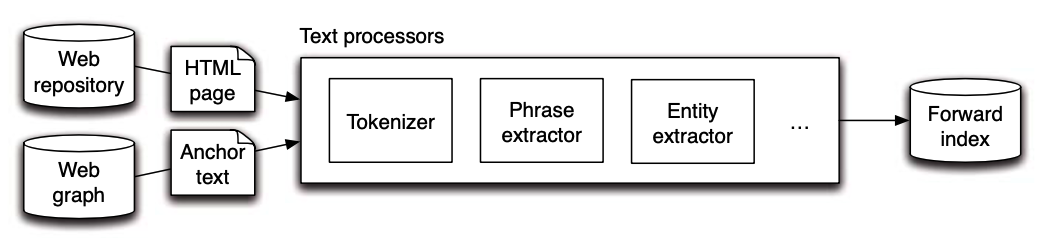
\includegraphics[width=0.7\textwidth]{figures/forward_index.png}
    \caption{Forward index}
\end{figure}
\begin{itemize}
    \item anchor text comes from links
    \item forward index: for every document store all informtion about the document (e.g. all the words that occur etc.)
\end{itemize}
\subsection{Page attribute file}
\begin{figure}[ht]
    \centering
    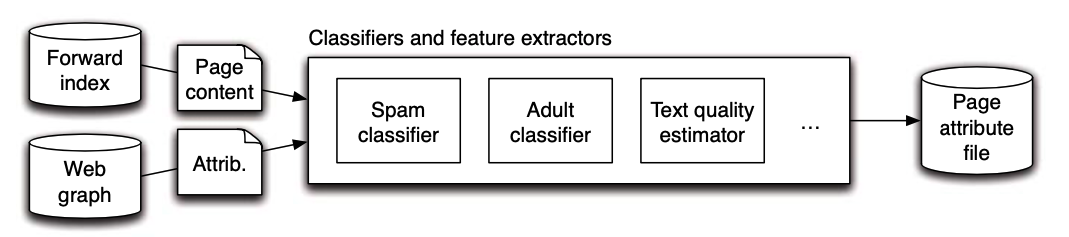
\includegraphics[width=0.7\textwidth]{figures/page_attribute_file.png}
    \caption{Page attribute file}
\end{figure}
\begin{itemize}
    \item Contains information such as language, length, text quality, link quality etc.
    \item whatever data describes the document, put it into a separate attribute file
\end{itemize}
\subsection{Inverted index}
\begin{figure}[ht]
    \centering
    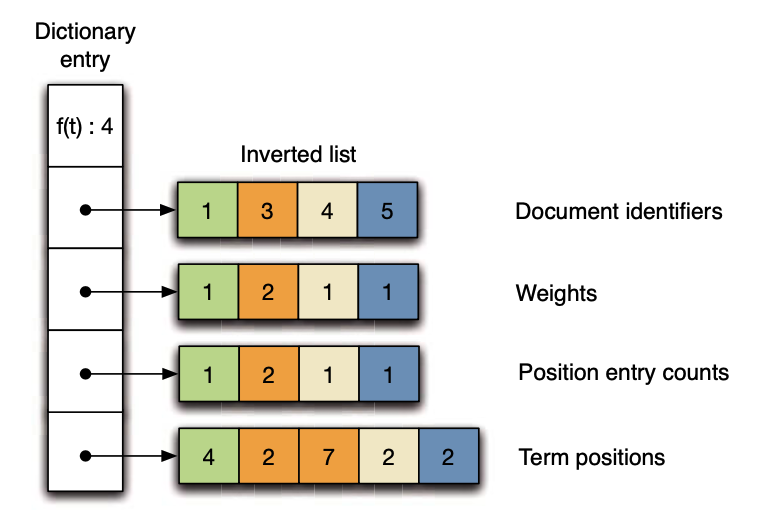
\includegraphics[width=0.5\textwidth]{figures/inverted_index.png}
    \caption{Full inverted index}
    \label{inverted_index}
\end{figure}
\begin{itemize}
    \item needed for search: from words to documents (e.g. index at the end of textbook)
    \item Inverted index is a dictionary where each entry contains total number of docs containing the term, pointer to start of the inverted list (which contains the document identifiers), other meta-data about the term
    \item the actual inverted list could be modelled by a B+-tree or hash table
    \item inverted list can also contain term-frequency per document or positions of the terms
    \item in reality, store all kinds of information in different inverted lists (e.g. one list for document identifiers, one list for term positions etc.)
\end{itemize}
See Fig. \ref{inverted_index}.

\subsection{Constructing inverted indices}
A simple construction algorithm that iterates through the documents and constructs an inverted index along the way has two problems: it is in-memory and is single-threaded.
Possible alternatives are:

\subsubsection{Two-pass index}
Addresses the in-memory issue.
\begin{figure}[ht]
    \centering
    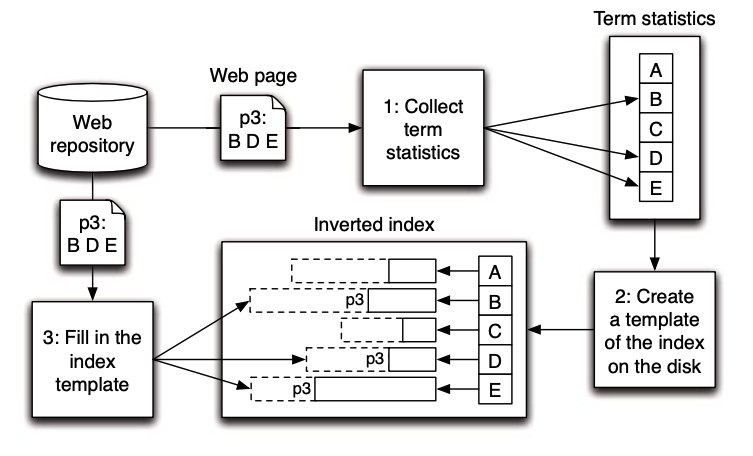
\includegraphics[width=0.5\textwidth]{figures/two-pass_index.png}
    \caption{Two-pass index}
\end{figure}
\begin{itemize}
    \item goes throught he collection two times
    \item first time, it computes statistics: for term A there are 10 documents etc.
    \item based on these statistics, empty index is created on disk
    \item during second pass, fill in the created indices
    \item -> use no RAM
\end{itemize}

\subsubsection{One-pass index with merging}
Addresses the in-memory issue.
\begin{figure}[ht]
    \centering
    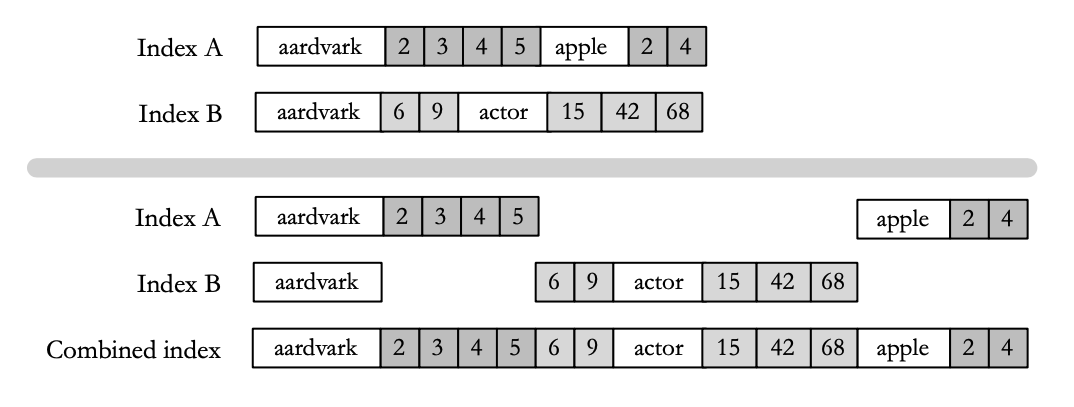
\includegraphics[width=0.7\textwidth]{figures/one-pass_index_merge.png}
    \caption{One-pass index with merging}
\end{figure}
\begin{itemize}
    \item construct multiple indices over possibly different documents until memory is full
    \item then merge the indices
    \item in some sense this is two passes as well
\end{itemize}

\subsubsection{Distributed indexing}
Addresses the single-threaded issue.
\begin{figure}[ht]
    \centering
    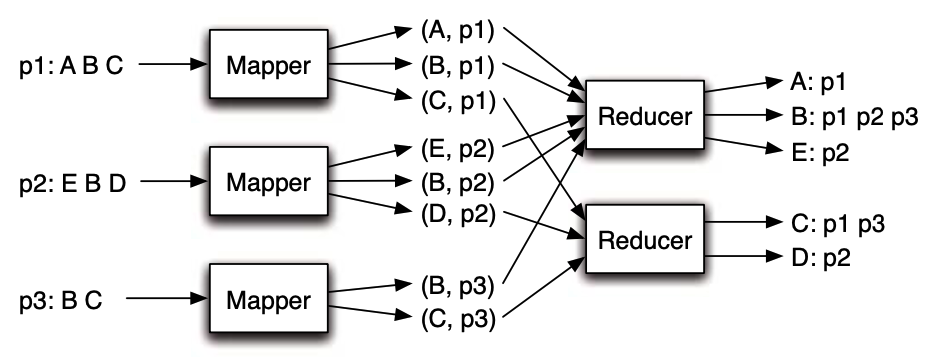
\includegraphics[width=0.5\textwidth]{figures/map_reduce.png}
    \caption{Distributed indexing (MapReduce)}
\end{figure}
\begin{itemize}
    \item two types of processes: maps and reduces
    \item take one mapper for each document -> process documents in parallel
    \item mapper produces pair of key = term and value = document
    \item reducers collect entries that have the same key and produces list of documents for each key
\end{itemize}

\subsection{Updating indices}
\subsubsection{No merge}
\begin{itemize}
    \item low index maintenance cost
    \item high query processing cost
    \item when encountering changes, add changes to delta index in memory
    \item when out of memory, flush delta to disc
    \item at query time, search all delta indices and merge
\end{itemize}
\begin{figure}[ht]
    \centering
    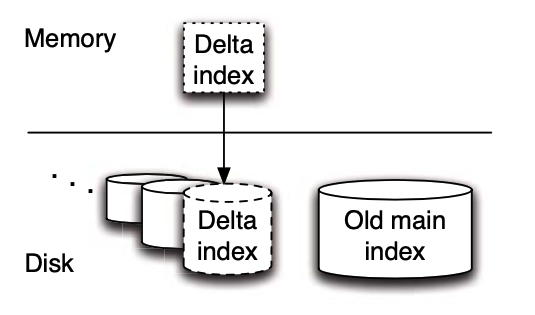
\includegraphics[width=0.4\textwidth]{figures/index_no_merge.png}
    \caption{Updating indices with no merge}
\end{figure}

\subsubsection{Incremental update}
\begin{itemize}
    \item keeps free buffer space
    \item no read/write of entire index when updating
    \item inverted lists are accessed concurrently as index querying and updating is done at the same time
    \item run out of free buffer space
\end{itemize}
\begin{figure}[h!]
    \centering
    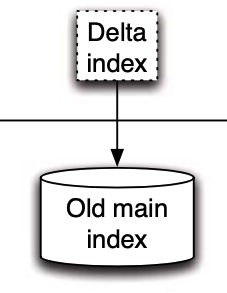
\includegraphics[width=0.15\textwidth]{figures/index_incremental_update.png}
    \caption{Updating indices with incremental updates}
\end{figure}

\subsubsection{Immediate merge}
\begin{itemize}
    \item always a single index
    \item read/write of entire index when updating -> slow when having many documents
    \item query only main index
\end{itemize}
\begin{figure}[ht]
    \centering
    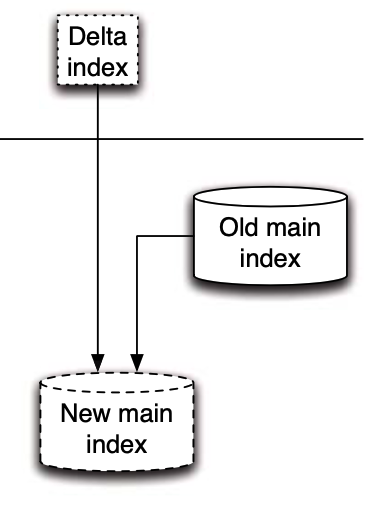
\includegraphics[width=0.2\textwidth]{figures/index_immediate_merge.png}
    \caption{Updating indices with immediate merge}
\end{figure}

\subsubsection{Lazy merge}
\begin{itemize}
    \item trade-off between index maintenance cost and query processing cost
    \item -> we have more than one index but not as many as first generation delta indices
    \item no concurrency
    \item -> practicals
\end{itemize}
\begin{figure}[ht]
    \centering
    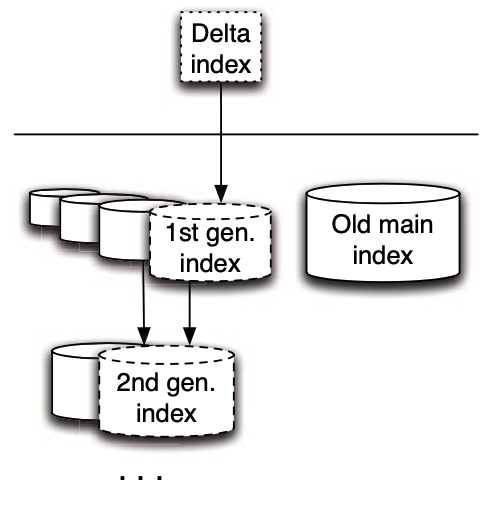
\includegraphics[width=0.3\textwidth]{figures/index_lazy_merge.png}
    \caption{Updating indices with lazy merge}
\end{figure}
